\documentclass{article}
\usepackage{tikz}
\usepackage{comment}
\usetikzlibrary{shapes,arrows}
\tikzstyle{line}=[draw]

\begin{document}

 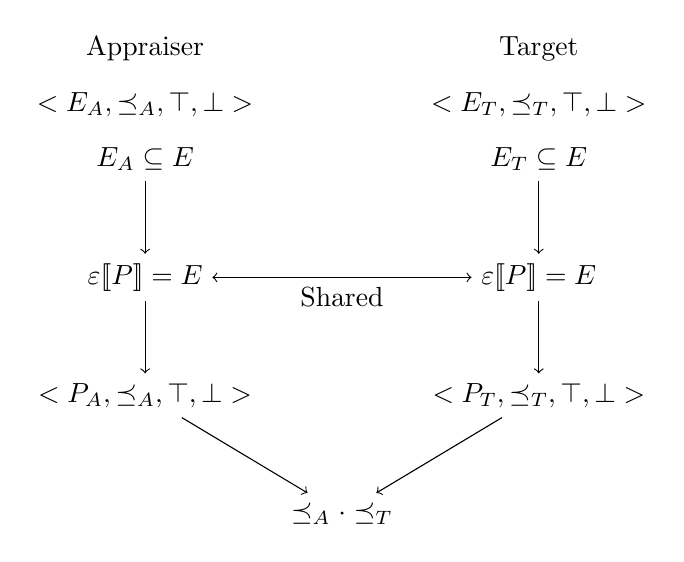
\begin{tikzpicture}

\node(A) {Appraiser};
\node (T) [node distance=5.0cm, right of=A]{Target};
\node (Ea) [node distance =7.0mm, below of=A] {$<E_{A},\preceq_A,\top,\bot>$};
\node (EaUniverse) [node distance =7.0mm, below of=Ea] {$E_A \subseteq E$};
\node (Et) [node distance=5.0cm, right of=Ea] {$<E_{T},\preceq_T,\top,\bot>$};
\node (EtUniverse) [node distance=5.0cm, right of=EaUniverse] {$E_T \subseteq E$};

\node(EvSemA) [node distance =1.5cm, below of=EaUniverse]{$\varepsilon [\![P]\!] = E$};
\node(EvSemT) [node distance =1.5cm, below of=EtUniverse]{$\varepsilon [\![P]\!] = E$};

\node(Pa) [node distance =1.5cm, below of=EvSemA]{{$<P_{A},\preceq_A,\top,\bot>$}};
\node(Pt) [node distance =1.5cm, below of=EvSemT]{$<P_{T},\preceq_T,\top,\bot>$};

\node(SharedOrderTemp) [node distance=1.5cm, below of=Pa]{};
\node(SharedOrder) [node distance=2.5cm, right of=SharedOrderTemp]{$\preceq_A \cdot  \preceq_T$ };


\draw [<->] (EvSemA) -- node[below] {Shared} ++ (EvSemT);
\draw [->] (EaUniverse) -- (EvSemA);
\draw [->] (EvSemA) -- (Pa);

\draw [->] (EtUniverse) -- (EvSemT);
\draw [->] (EvSemT) -- (Pt);

\draw [->] (Pa) -- (SharedOrder);
\draw [->] (Pt) -- (SharedOrder);


\end{tikzpicture}

\vspace{8mm}
$\preceq_A, \preceq_T = $ negotiation
\newline \indent $\preceq_A \cdot  \preceq_T = $ selection policy
\newline \indent $E_T =\{e : E | \pi_T(e)\} = $ privacy policy
\newline \indent $\pi_T $ and $\pi_A $ are privacy policies for the target and appraiser, respectively
\end{document}